%! TEX root = ../main.tex
\documentclass[main]{subfiles}
\usepackage{adjustbox}

\begin{document}
\chapter{提案手法}
\section{DCASE基礎モデル}
\subsection{音響イベント検出 (SED)}
\label{DCASE基礎モデル:音響イベント検出}
DCASE 2024では、タスクとしてSEDを扱う。
% 解説用の図を作成する
\begin{figure}[!htbp]
    \centering
    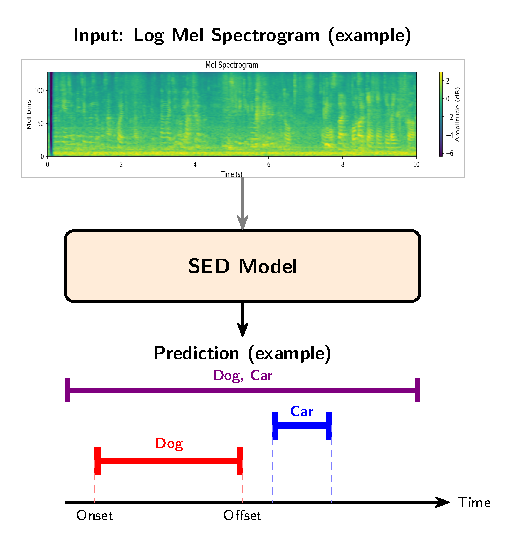
\includegraphics[width=80mm]{figures/sed.pdf}
    \caption{クリップ予測及びフレーム予測の、10秒の音声入力を対象とした出力例。全体におけるイベントの有無を判定するクリップ予測に対し、フレーム予測ではイベントの区間（Onset/Offset）も算出する。注: 入力のスペクトログラムと予測結果はあくまで構造を説明するためのイメージであり、実際の対応はない。}
    % 図の説明をより詳細にする。
    \label{fig:sed}
\end{figure}
\clearpage

本タスクでは、10秒間の音声データを「クリップ」、それをさらに短時間で分割した単位を「フレーム」と定義し、イベント種別及び各イベントの開始・終了時刻を予測する。
音声データ内（クリップ及びフレーム）では、複数のイベントが重複して発生する可能性があるため、SEDでは複数のイベント種別とその発生時刻を同時に予測することが求められる。
図\ref{fig:sed}に示すように、学習においてはクリップ単位では10秒間にどのイベントが含まれているか（イベントの有無）を、フレーム単位ではイベント種別に加えて、その開始・終了時刻（時間的境界）を学習対象とする。 \par

また、予測の粒度に応じてデータのラベル定義が異なる。時間的な詳細情報を含むものを「強ラベル」、イベントの有無のみを示すものを「弱ラベル」とし、それぞれフレームとクリップに対応する。

\subsection{データセット}
\label{DCASE基礎モデル:データセット}
本研究ではデータセットとして、DESEDとMAESTRO Realを用いる\cite{turpault2019sound, serizel2020sound, martin2023strong}。
そのうち、10（Alarm bell ringing、Blender、Cat、Dishes、Dog、Electric shaver toothbrush、Frying、Running water、Speech、Vacuum cleaner）及び11（Birds singing、Car、People talking、Footsteps、Children voices、Wind blowing、Brakes squeaking、Large vehicle、Cutlery and dishes、Metro approaching、Metro leaving）クラスを使用する。\par

DESEDのデータは学習の利用段階とデータの作成法、ラベルで分類される。利用段階には訓練、検証、評価がある。データは実環境の録音か、あるいは合成で作成され、ラベルは強、弱、なしに分類される。
ここで、ラベルの強・弱はフレーム・クリップに対応しており、フレームごとにイベントの開始・終了・種類が記録されていれば強ラベル、10秒のクリップに対して含まれるイベントの種類のみであった場合は弱ラベルに分類される。ラベルなしは全くラベルが付加されていないデータを指す。
なお、本研究では一部データが取得できず、通常より少ないデータ数で学習を行っている。本研究で使用したDESEDのデータ数は表\ref{table:desed}の通り。\par
\begin{table}[htbp]
 \begin{center}
   \begin{tabular}{|l|c|c|}
    \hline
    利用段階 & データ種別  & 数[clips] \\
    \hline
    訓練 & 強ラベル、実録音 & 1613 \\
    訓練 & 弱ラベル、実録音 & 1188 \\
    訓練 & 強ラベル、合成音 & 10000 \\
    訓練 & ラベルなし、実録音 & 12027 \\
    検証 & 弱ラベル、実録音 & 129 \\
    検証 & 強ラベル、合成音 & 2500 \\
    評価 & 強ラベル、実録音  & 958 \\
    \hline
  \end{tabular}
  \caption{データ数}
  \label{table:desed}
\end{center}
\end{table}

MAESTRO Realは実環境での録音が含まれるデータセットである。訓練用のデータを訓練と検証で9:1に分割し、評価には評価用のデータを用いた。

\clearpage

\subsection{全体の流れ}
モデル全体の流れは学習と検証、評価の三つに区別される。\par
学習から検証までの大まかな流れを図\ref{fig:flow_c}に示す。なお、図中の前処理は\ref{提案手法: 前処理}節で、モデルは\ref{DCASE:モデル構成}節で述べる。
前処理を行ったデータを用いて学習を150エポック行い、モデルは弱ラベルに対する予測（弱予測）と強ラベルに対する予測（強予測）を出力する。教師あり学習と、半教師あり学習による損失を各予測で計算した後、最適化アルゴリズムの一種であるAdam\cite{kingma2014adam}によって生徒モデルを、指数移動平均によって教師モデルを、それぞれ更新する。\par

検証は10エポックごとに行われる。学習したモデルを読み込み、検証用データに対して推論させ、その結果を用いて精度を計算する。過去の検証より精度が向上した場合、そのモデルの重みパラメータを保持する。\par
\begin{figure}[htbp]
    \centering
    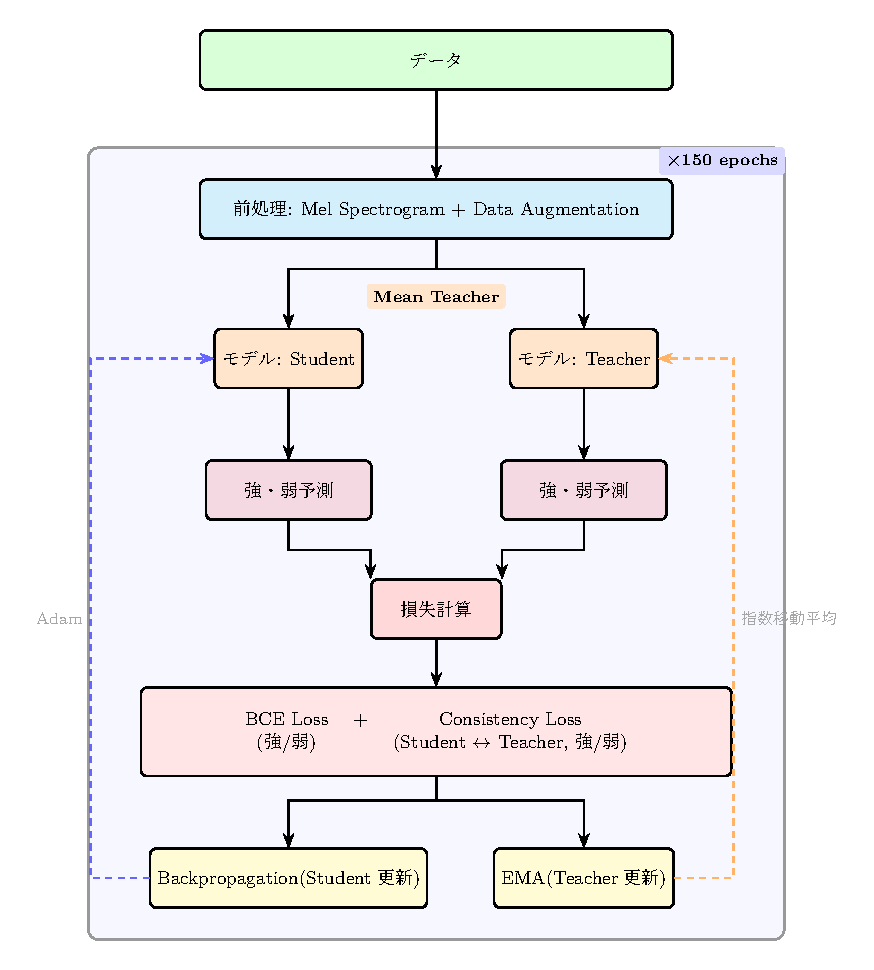
\includegraphics[width=110mm]{figures/flow_c_3.pdf}
    \caption{学習から検証の流れ。データの前処理とモデルの準備を行い、150エポックの学習を行う。検証は10エポックごとに行う。}
    \label{fig:flow_c}
\end{figure}

\clearpage

評価の流れを図\ref{fig:flow_eval}に示す。
評価は検証時に最高の精度を出したモデルを読み込み、評価用データに対して推論させ、精度を計算する。
ベースラインでは後処理にMedian Filterを用い、予測を平滑化する。モデルの直接的な出力は時間的な連続性が考慮されず、イベント検知が断片的になる。
そのため、イベント種別に応じたフィルタサイズで平滑化し、連続的なイベント区間として統合する。これに対し、提案手法では後処理手法としてSEBBsを採用する。詳しくは\ref{提案手法:SEBBs}節で述べる。

\begin{figure}[!htbp]
    \centering
    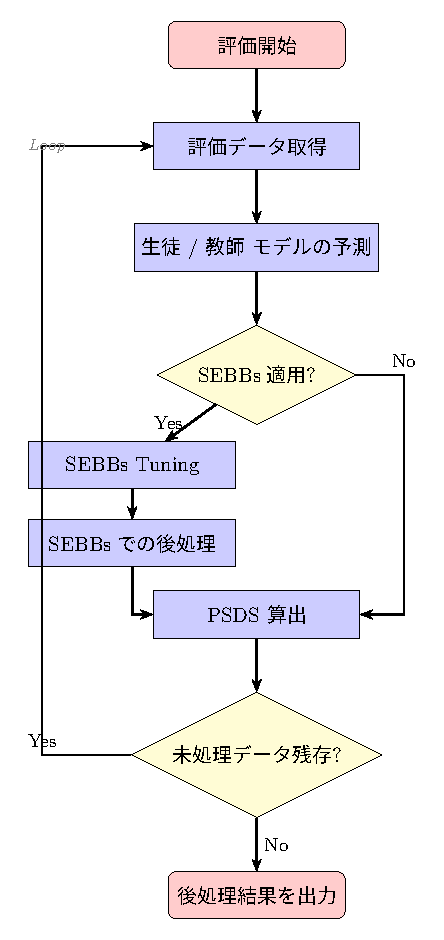
\includegraphics[width=80mm]{figures/flow_eval_2.pdf}
    \caption{評価の流れを表すフローチャート。SEBBsの使用可否で分岐する。}
    \label{fig:flow_eval}
\end{figure}

\clearpage

\subsection{前処理}
\label{提案手法: 前処理}
\begin{figure}[!htbp]
    \centering
    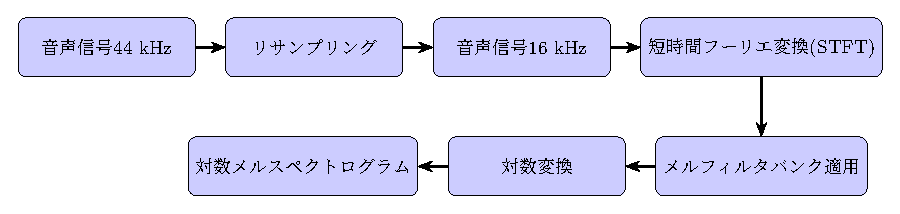
\includegraphics[width=120mm]{figures/pre.pdf}
    \caption{対数メルスペクトログラムを得るまでの流れ。この後、確率的にデータ拡張を適用する。}
    \label{fig:pre}
\end{figure}
本研究における音声データの前処理はDCASE 2024の公式設定に準拠し、図\ref{fig:pre}のように行う。
まず、サンプリング周波数44 kHzの音声信号を16 kHzへとリサンプリングし、計算負荷を低減しつつ、タスクに適した帯域に制限する。
次に、短時間フーリエ変換（STFT）を適用して時間周波数表現を得た後、
人間の聴覚特性を模したメルフィルタバンクによって、周波数軸をメル尺度（Mel scale）へと変換。
最後に、得られたメルスペクトログラムに対し、信号のダイナミックレンジ（信号の強さの幅）を圧縮してモデルの学習安定性を高めるため、
パワー（振幅の二乗）に対して対数変換を施し、対数メルスペクトログラム（Log-Mel Spectrogram）を算出する。
\par

\newpage

図\ref{fig:pre_eg}に前処理の各段階のデータを可視化した。
横軸はいずれも音声データの時間を、縦軸は上から振幅、周波数、メル周波数を表し、スペクトログラムの色は振幅の大きさを表す。
図\ref{fig:pre_eg}より、STFTによって振幅の強さが各周波数と時間によって取り出され、それがメルフィルタバンクによって変換されることが分かる。
\par

\begin{figure}[!htbp]
    \centering
    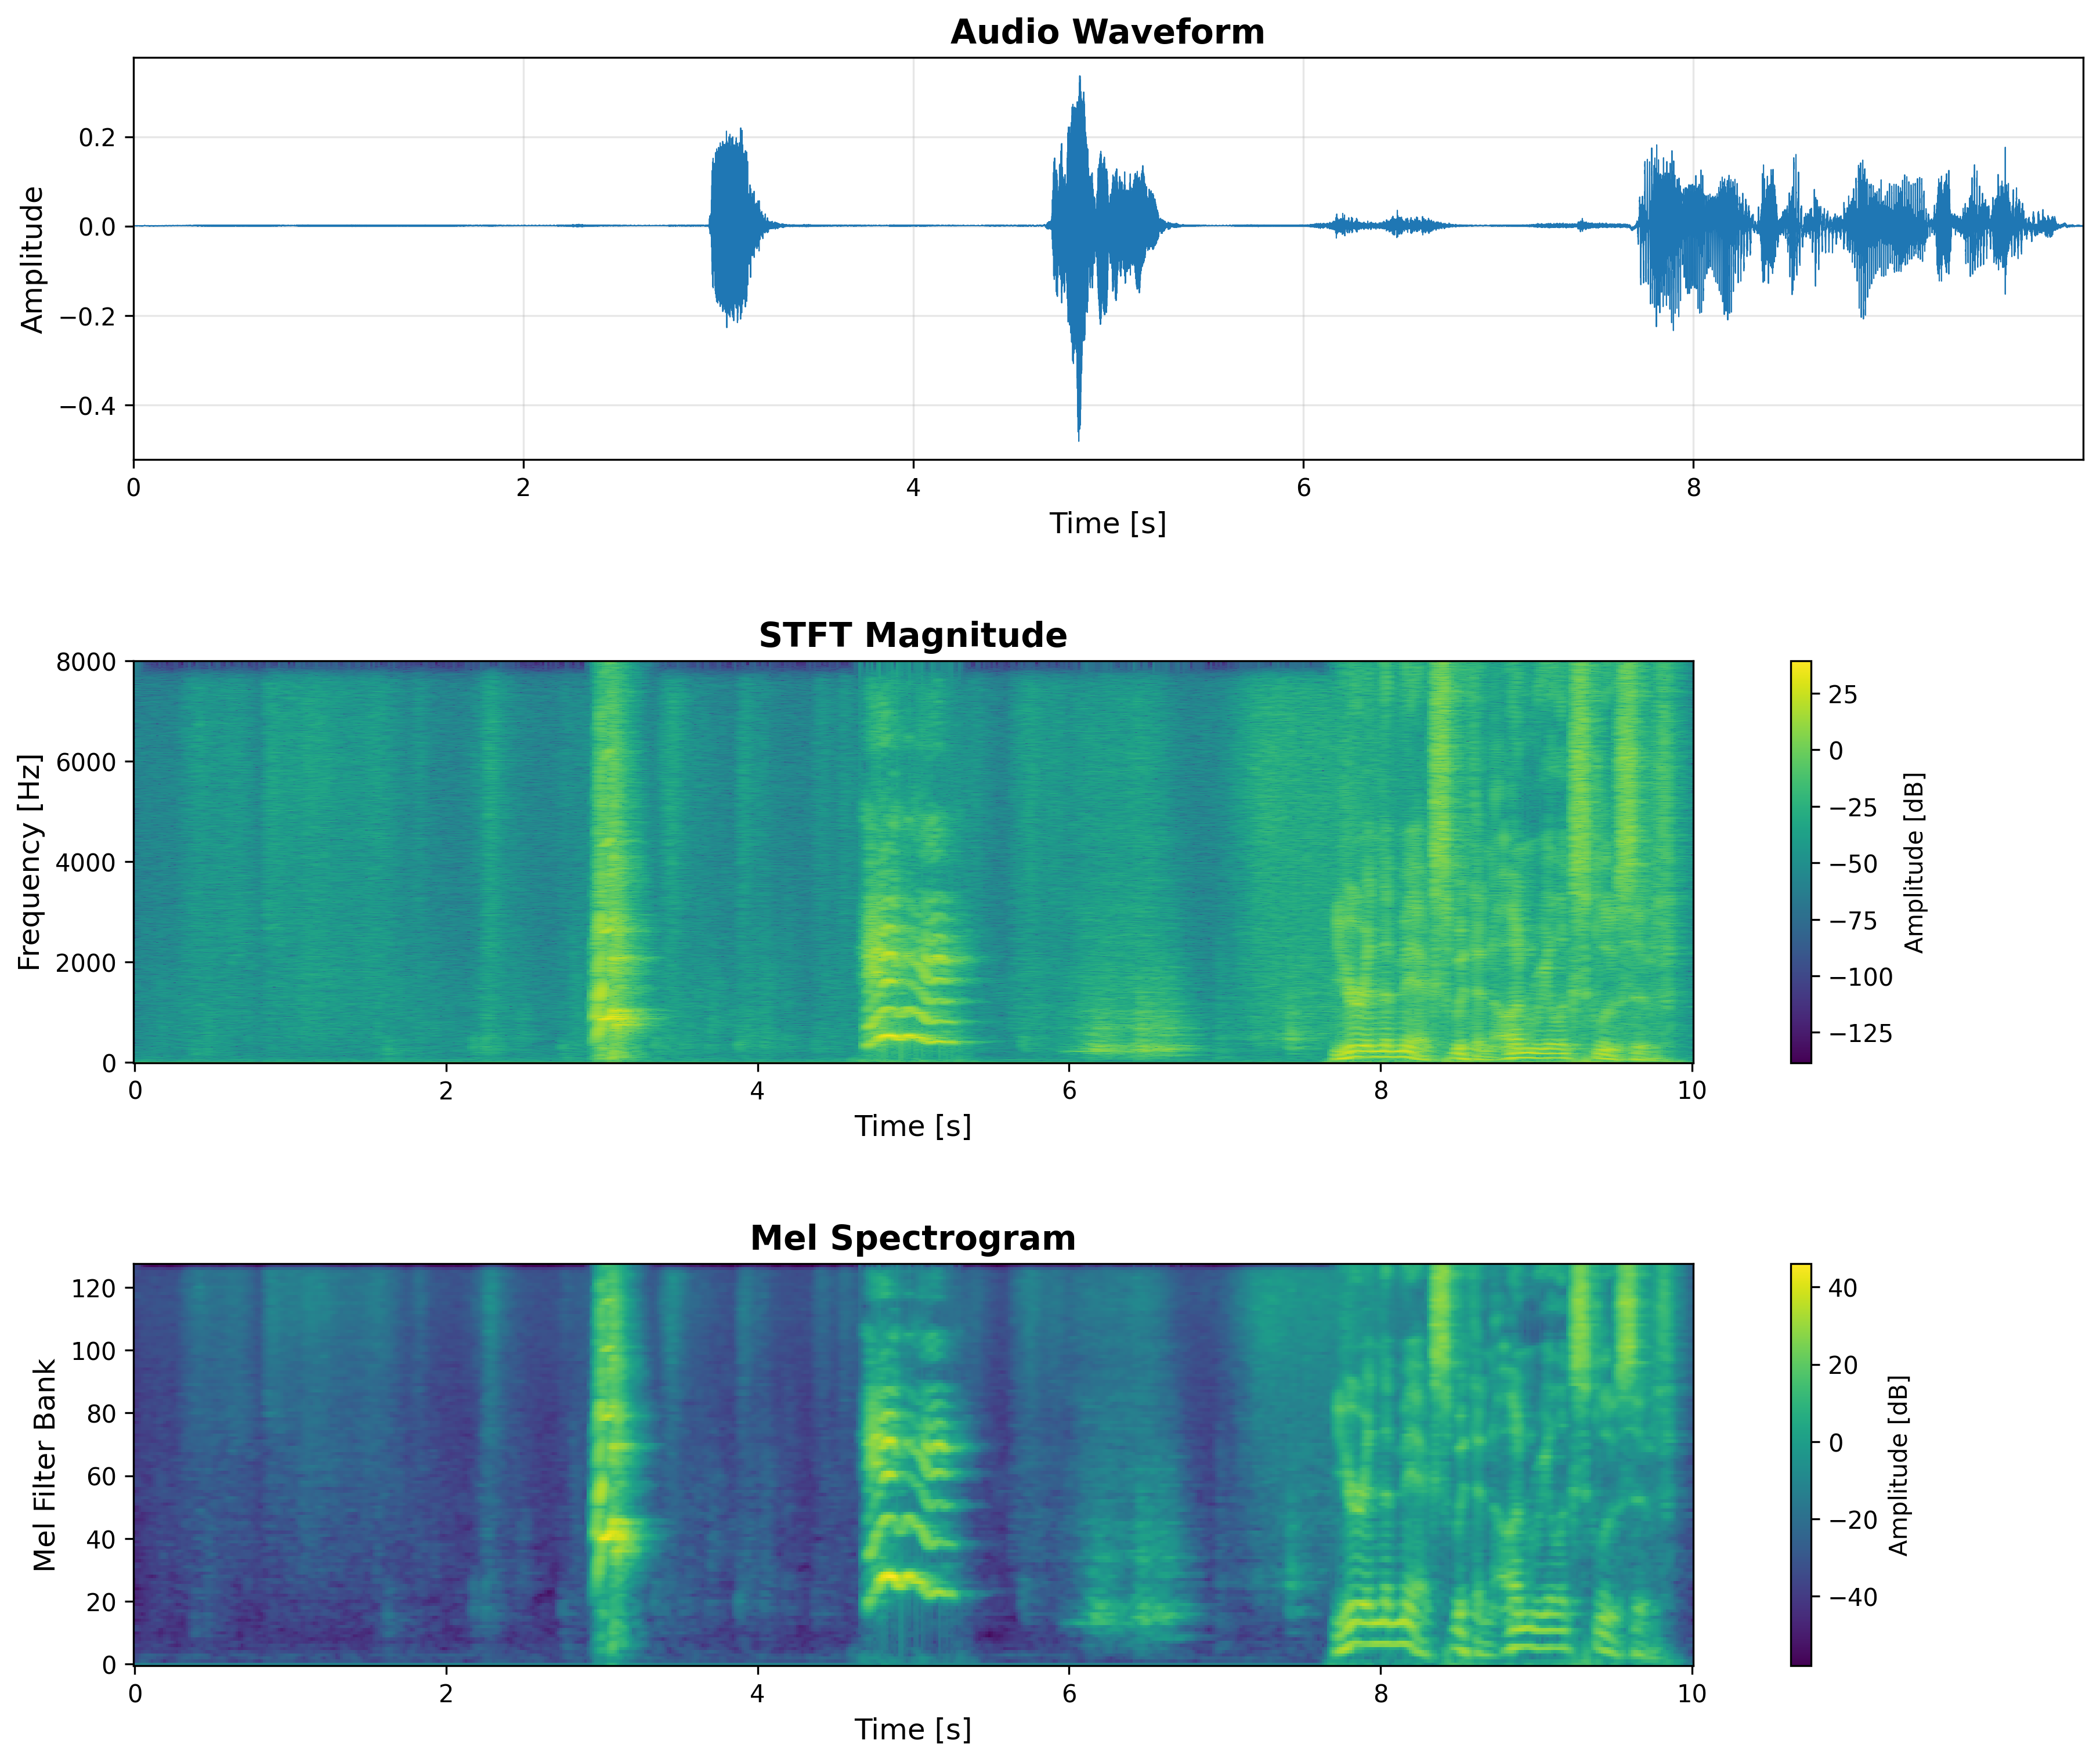
\includegraphics[width=120mm]{figures/preprocessing.png}
    \caption{音声データを可視化した。それぞれ生音声、短時間フーリエ変換後、メルフィルタバンク通過後を表す。}
    \label{fig:pre_eg}
\end{figure}

その後、データに対してMixupを適用する\cite{zhang2017mixup}。
Mixupは、2つの学習データとそのラベルをベータ分布からサンプリングされた比率で凸結合（重み付き和で混合）し、新たな訓練サンプルを生成することで、モデルの汎化性能を向上させるデータ拡張手法である。

\clearpage

\subsection{モデル構成}
\label{DCASE:モデル構成}
\begin{figure}[htbp]
    \centering
    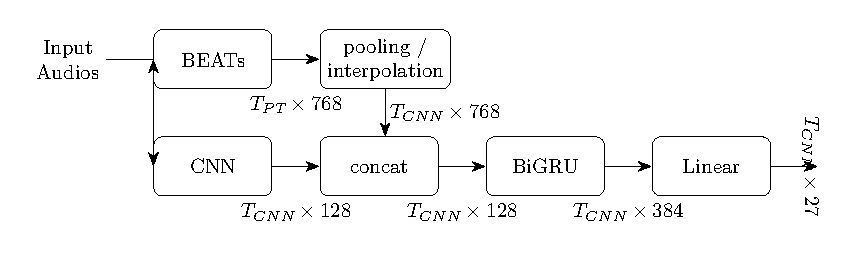
\includegraphics[width=150mm]{figures/model.pdf}
    \caption{先行研究で使用されたモデル。各段階の次元数は、特徴量の時間長 (フレーム数) と周波数を表す。BEATsによる埋め込みをプーリングや補間によって調整し、CNNの出力と統合。RNN（BiGRU）に入力した後、確率値からクリップ及びフレーム予測を得る。なお、T: 時間長, PT: 事前学習済みモデルとする。}
    % 図の説明をより詳細にする。
    \label{fig:model}
\end{figure}

DCASE 2024のベースラインモデルの大まかな構成を図\ref{fig:model}に示す。
本モデルは、時間周波数領域の局所的な特徴を抽出するCNNと、時系列情報を学習しイベントの時間的変化をモデル化する再帰型ニューラルネットワーク（Recurrent Neural Network; RNN）を組み合わせた、CRNN（Convolutional Recurrent Neural Network）アーキテクチャを採用している。
また、特徴抽出器として、事前学習されたBEATs（Bidirectional Encoder representation from Audio Transformers）\cite{chen2022beats} を導入している。
事前学習済みモデルの活用により、学習コストを抑制しながらタスクに有効な特徴表現を獲得することが期待される。
詳細な設定については、DCASE 2024に準拠する。\par

% ここで、図\ref{fig:model}中の$T_{CNN}$、$T_{PT}$について説明する。これらは時間フレーム数を表す。CNNは16kHzを256ホップで処理するため625フレームとなるが、
% BEATsはFbank 特徴量を扱い, CNNと時間フレーム数が合わない。そこで、

モデル内における各データの次元数及び処理フローは以下の通りである。\par
まず、入力音声からBEATsを経て得られた埋め込み特徴量（$T_{PT} \times 768$）は、プーリング及び補間処理（Pooling / Interpolation）によって時間解像度が調整される。
なお、BEATsへの入力は事前学習時と一貫性を保つため対数変換せず、フレーム数もCNNと異なる。\par

次に、調整されたBEATsの特徴量（$T_{CNN} \times 768$）は、CNNから得られる特徴量（$T_{CNN} \times 128$）と結合（Concat）される。
そして、結合された特徴量はBiGRU層に入力され、最終的に全結合層（Linear）などの出力部を介して、時間とクラス数に基づいた予測値（$T_{CNN} \times 27$）として出力される。
これにより、クリップ単位及びフレーム単位でのイベント検出が可能となる。\par

\subsubsection{CNN}
本モデルのCNN部は、図\ref{fig:cnn}に示す通り7つの畳み込みブロックで構成されており、その設定はDCASE 2024に準拠する。
各ブロックは、Conv2D、Batch Normalization、ReLU、Dropout、及びMaxPool2Dを順に積層した構造になっている。\par

\begin{figure}[htbp]
    \centering
    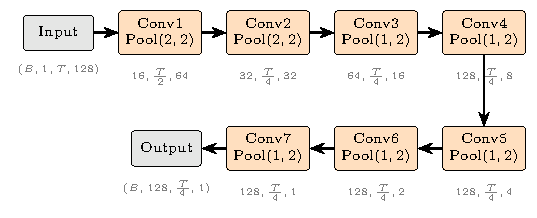
\includegraphics[width=100mm]{figures/cnn_3.pdf}
    \caption{CNNの構造を示す。畳み込み層を含んだブロックが7つあり、これらは役割に応じて三種類に大別される。各要素の下の数値は特徴量の次元数（バッチ数、チャネル数、時間長 (フレーム数) 、周波数）を表す。}
    \label{fig:cnn}
\end{figure}

これらのブロックは、その役割に応じて以下の3段階に分類される。便宜上、7つのブロックを上からブロック1、2、...と呼称する。\par
まず、ブロック1-2で基礎的な特徴抽出のため、時間及び周波数の両解像度を段階的に圧縮する。
次に、ブロック3-4では特徴の増強を目的に、時間方向の解像度を維持しつつ、音響イベントの識別に必要な周波数情報の集約を行う。
最後に、残りのブロックは周波数次元をさらに圧縮し、意味的な高次特徴へと変換する。\par
こうして得られたCNNの出力は、周波数次元を平坦化した後、BEATsの埋め込み特徴量と結合される。
この設計により、CNNが捉える局所的なスペクトログラムの変化と、BEATsが有する広範な音響的文脈情報の双方を活用することが可能となる。\par


\newpage

\subsubsection{RNN}
RNN部には、双方向Gated Recurrent Unit（Bidirectional GRU; BiGRU）を使用する (図\ref{fig:rnn}) 。
BiGRUは順方向と逆方向に特徴を処理することで、イベントの時間的な変化を学習する。
本構成はDCASE 2024の設定に準拠している。\par
処理の流れとして、入力特徴量に対して時間軸方向にランダムなマスキングを行った後、Dropout、BiGRU、Dropoutと順に適用し、最終的な特徴量を得る。

\begin{figure}[htbp]
    \centering
    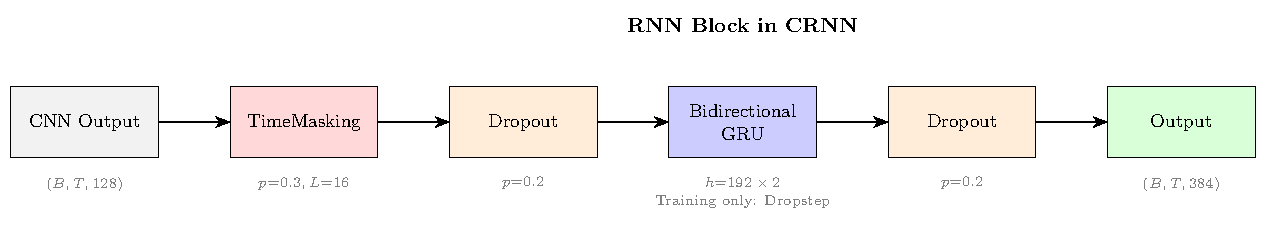
\includegraphics[width=150mm]{figures/rnn_2_horizontal.pdf}
    \caption{RNNの構造を示す。CNNからの入力を受け取ってTime Masking・Dropoutと順に適用し、BiGRU層に入力した後、再度Dropoutを適用する。なお、図中のhはRNNの隠れ層の数を表す。}
    \label{fig:rnn}
\end{figure}

\subsubsection{予測の出力}
\begin{figure}[htbp]
    \centering
    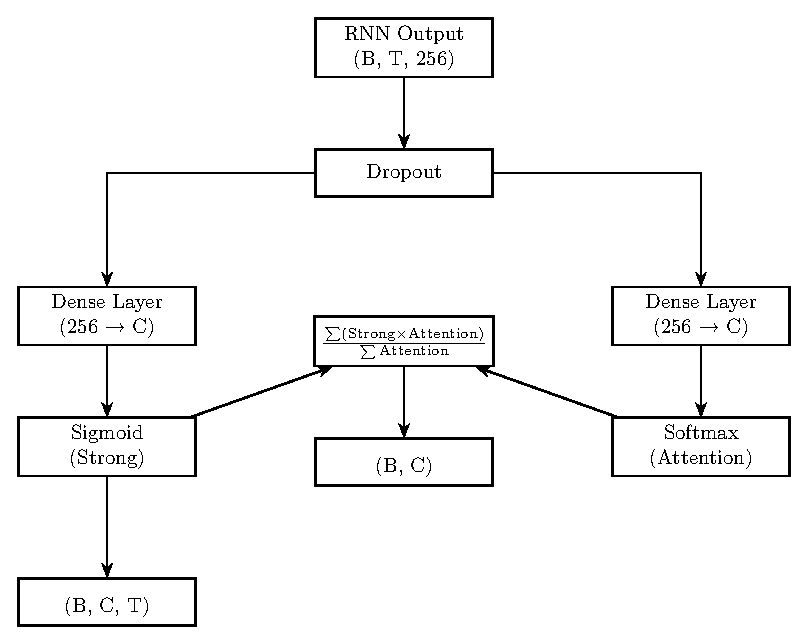
\includegraphics[width=110mm]{figures/linear_2.pdf}
    \caption{出力の構造を示す。各文字について、B: バッチ数、C: クラス数、T: 時間長（フレーム数）を表す。}
    \label{fig:linear}
\end{figure}

本モデルの出力段は、RNNからの出力（$\text{Batch} \times \text{Time} \times 384$）を入力とし、以下のプロセスを経てフレーム（強）及びクリップ（弱）予測を行う。\par
まず、RNNの出力は全結合層（Linear Layer）とSigmoid活性化関数を通り、27クラスに対する強予測へと変換される。
次に、弱予測を得るため、Attention機構による時間方向の集約を行う。
具体的には、並列した全結合層とSoftmax関数を用いて時間方向のAttention重みを算出し、これを用いた強予測の重み付き平均を最終的な弱予測とする。
なお、評価時には前述の21クラスの予測を使用する。

\section{Mean Teacher}
\label{提案手法:CMT}
\begin{figure}[!htbp]
    \centering
    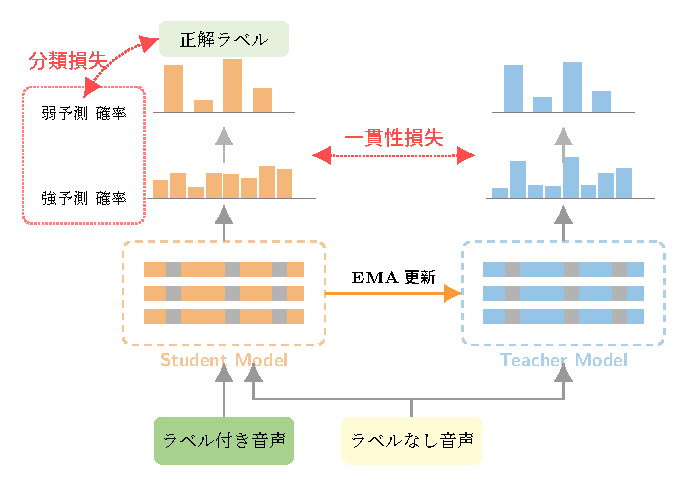
\includegraphics[width=120mm]{figures/mt_sed.pdf}
    \caption{Mean Teacherの更新の概略。Mean TeacherはDESEDに対して適用し、生徒モデルの重みパラメータの指数移動平均で教師モデルのパラメータを更新する。Model内の灰色部は、モデルの一部にDropOutが適用され、ノイズ (摂動)として働くことを表す。}
    \label{fig:meanteacher}
\end{figure}


\subsection{Mean Teacherと一貫性損失}
Mean Teacherは、一貫性正則化（Consistency Regularization）に基づく半教師あり学習手法である。
通常の学習を行うモデルを「生徒（Student）」とし、その重みパラメータの指数移動平均を用いて、
より挙動の安定した「教師（Teacher）」モデルを構築する。
教師モデルは、入力データに対する自身の予測を疑似ラベル（Pseudo-label）として提供し、生徒モデルを導く役割を果たす。
具体的には、入力に対して摂動（ノイズ等）が加えられた場合でも、教師と生徒が同様の予測を出力することを仮定し、
両者の予測間の差異を「一貫性損失（Consistency Loss）」として定義する。
ベースライン手法では、この損失関数に平均二乗誤差（MSE）を用いる。
ここで、DESEDは強ラベル、弱ラベル、ラベルなしのデータがあるが、ラベルなしでは一貫性損失のみを利用し、ラベル付きには教師あり学習の損失（MSE）と一貫性損失の双方を用いて学習を行う。\par

\subsection{Confident Mean Teacher}
Confident Mean Teacher (CMT) は、Mean Teacherにおける疑似ラベルに誤りが含まれる可能性を考慮し、信頼度の高い予測のみを選別して学習に用いる手法である。
具体的には、クリップ単位及びフレーム単位で閾値を設け、これを超過した予測のみを信頼できるとみなすフィルタリング処理を行う。 \par
CMTの処理手順は以下の通りである。まず、クリップレベルの予測（弱予測）に対し信頼性を判定する。
閾値を下回る（信頼できない）場合は、そのクリップ内の全フレーム予測（強予測）も信頼できないとみなし、学習から除外する（値を0とする）。
次に、信頼できるとされたクリップ内のフレーム予測に対して再度、閾値を判定する。
さらに、イベント種別に応じた窓サイズを持つMedian Filterを適用することで、予測の平滑化と外れ値の除去を行う。 
最終的な損失計算では、二値化された信頼度マスクを重みとして教師の予測に適用し、教師と生徒の予測間での二値交差エントロピー（Binary Cross Entropy; BCE）を最小化する。\par

\subsection{提案手法：負例を活用した $CMT_{neg}$}
本研究において従来のCMTを再現実装したところ、イベント検知の評価指標であるPSDS2は向上したものの、時間的な境界の精度（時間分解能）を重視するPSDS1が低下した。
これは、CMTが閾値以下の予測を損失計算から完全に除外するため、確信度の低い予測、すなわち「イベントが存在しない（負例）」という情報が学習に活用されていないことに起因すると考えられる。
その結果、時間分解能が低下したと解釈できる。\par
そこで本稿では、負例を明示的に学習に組み込むことで、PSDS2の改善を維持しつつPSDS1を回復させる手法 $CMT_{neg}$ を提案する。
具体的には、予測確率が高い（例：0.7以上）データを「信頼できる正例」、予測確率が低い（例：0.3以下）データを「信頼できる負例」と定義し、中間領域の、モデルの自信が曖昧な予測を除外する。
これにより、ラベルなしデータにおける背景（イベントなし）情報を有効活用する。\par
さらに、正例と負例のサンプル数に偏りが生じないよう、量の少ない方に合わせてサンプリングを行う均衡化処理を導入した。
検証の結果、提案手法である均衡化を含んだ $CMT_{neg}$ （$CMT_{scale}$ ）は、PSDS1においてMean Teacherと同等の性能を維持しつつ、PSDS2においてはCMTを上回る性能を達成した。\par


\section{MixStyle}
\label{提案手法:MixStyle}

MixStyleは本来、画像認識分野においてドメイン汎化を目的として提案されたデータ拡張手法である。
画像におけるMixStyleは、空間情報に着目しチャネル方向で統計量を混合する。
一方で、音響信号は時間と周波数の次元を持ち、ドメイン情報は主に周波数領域に局在することが示唆されている\cite{kim2022domain}。
この特性を踏まえ、Xiaoら\cite{xiao2024fmsg}は時間方向の平均と分散を計算し、周波数軸に沿って統計量を混合する手法を採用している。
これにより、元のデータに含まれる意味的な情報を保持しつつ、新たなドメインスタイルを持つデータを生成し、モデルが特定ドメインに過剰適合することを防ぐ。\par

しかし、先行研究\cite{xiao2024fmsg}ではMixStyleと周波数注意機構の結合が試みられているものの、
その具体的な統合プロセスや相互作用に関する詳細な記述が不足している。
そこで本研究では、周波数領域におけるドメイン汎化性能を最大化するため、MixStyleと軽量なCNNを明示的に統合する新たなアーキテクチャ（図\ref{fig:mixstyle}）を提案する。
本手法は以下の3段階で構成される。 
\begin{enumerate}
\item CNNによる重要周波数帯域の特定 
\item 重要度を考慮した重み付き統計量の混合 
\item 残差接続による原信号のドメイン情報の保持 
\end{enumerate}

これらにより、重要な信号情報を損失することなく、効果的なドメイン適応を実現する。\par
\begin{figure}[!htbp]
    \centering
    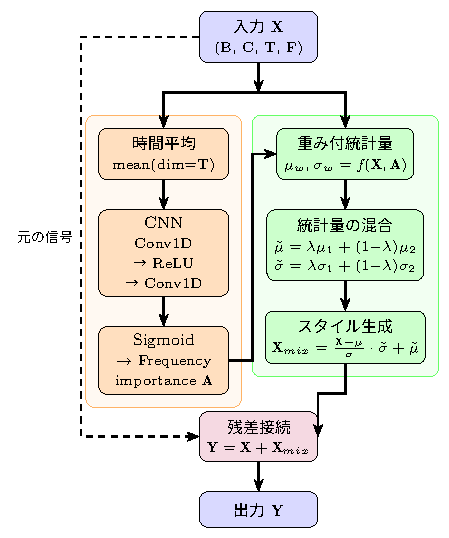
\includegraphics[width=100mm]{figures/mixstyle.pdf}
    \caption{オレンジの領域がCNN、緑がMixStyle、そして赤が残差接続で、それぞれ本文の1から3に対応する。}
    \label{fig:mixstyle}
\end{figure}


MixStyleの適用箇所は\cite{xiao2024fmsg}に準拠し、CNNへの入力直前の特徴量、及び第1・第2畳み込み層の直後の計3箇所とした。図\ref{fig:cnn}ではInput、ブロック1、2の後となる。
ハイパーパラメータは\cite{zhou2021domain}を参考に、適用確率を$p=0.5$、ベータ分布のパラメータを$\alpha=0.1$と設定した。
混合するスタイルのソースとなるデータは、ミニバッチ内からランダムに選択される。
本実験では汎化対象としてDESED（合成音）とMAESTRO Real（実録音）を使用しているが、
MixStyleはランダムなシャッフルであっても十分な正則化効果が得られることが報告されているため、計算コストと実装の複雑性を考慮し、バッチ内ランダム選択を採用した。\par

提案手法を具体的に説明する。入力特徴量を $X \in \mathbb{R}^{B \times C \times T \times F}$ とする（$B, C, T, F$ はそれぞれバッチサイズ、チャネル数、時間、周波数の次元を表す）。
まず、時間方向に対して平均を取り、時間情報を集約した周波数特徴記述子 $Z \in \mathbb{R}^{B \times C \times F}$ を得る。
$$Z_{b,c,f} = \frac{1}{T} \sum_{t=1}^{T} X_{b,c,t,f}$$

続いて、この特徴量に対して軽量なCNNを適用し、周波数ごとの重要度マップ $A \in \mathbb{R}^{B \times C \times 1 \times F}$ を生成する。
具体的には、カーネルサイズ3の1次元畳み込み層、ReLU活性化関数、及びカーネルサイズ1の畳み込み層からなるボトルネック構造を採用した。
最終層にはSigmoid関数を適用し、値域を $(0, 1)$ に正規化している。
$$A = \sigma(W_2 \cdot \delta(W_1 \cdot Z))$$

ここで $\delta$ はReLU関数、$W_1, W_2$ は畳み込み層の重みを表す。
学習の初期段階における勾配消失を防ぎ、混合を促進するため、最終層のバイアスは $1.0$ で初期化した。

推定された重要度 $A$ を用いて、重み付き平均 $\mu$ 及び重み付き標準偏差 $\sigma$ を算出する。
これらを用いて正規化及び異種ドメイン（バッチ内の他データ）の統計量との混合を行い、新たな特徴量 $X_{mix}$ を生成する。
最後に、元の信号情報の損失を防ぐため、生成された特徴量を残差成分として元の入力に加算する。
$$Y = X + \text{MixStyle}(X, A)$$
この残差構造により、モデルは元の信号に含まれる重要なイベント情報を保持しつつ、MixStyleによるドメイン変動への頑健性を学習することが可能となる。\par

実験ではCNNによる精度の向上が確認されたが、現在の実装は時間軸の平均と分散の計算時に重みづけをしており、期待される効果が発揮されていない可能性がある。
よって、実際にはCNNではなく残差接続により、元の特徴を維持しつつ摂動が加わったので、精度が向上したと考えられる。


\section{Sound Event Bounding Boxes}
\label{提案手法:SEBBs}
SEDにおいて、モデルは通常フレーム単位の確率値を出力するため、これをイベント単位の検出結果として評価するには、連続するフレームを統合する後処理が不可欠である。
従来、この後処理には主にMedian Filterが用いられてきた。
この手法は、クラスごとに固定された窓幅を用いて平滑化を行うものであるが、窓幅の調整が手動である点や、未知のイベント長への適応が困難であるという課題があった。
これに対し、SEBBsは、データから各クラスのイベント長を考慮して予測を整形する手法である。
本研究では、特に変化点検出に基づいてイベント境界を最適化するcSEBBs（change-point based SEBBs）を採用する。\par

本実験において、cSEBBsのハイパーパラメータは検証データを用いて最適化し、その設定を評価データへの適用時に使用した。
なお、パラメータのチューニングはデータセット（DESED及びMAESTRO Real）及びモデル（生徒・教師モデル）の組み合わせごとに個別に行った。
これは、各データセットで用いる評価指標が異なることと、より安定した教師だけでなく生徒の出力も観察しようと考えたからである。
しかし、推論に用いるのはより精度の高い教師であるため、評価の際は教師の結果のみを論じる。
\end{document}